\documentclass[a4paper,12pt]{article}
\usepackage{graphicx}
\begin{document}
\author{}
\title{Harvest Requirements and Design Documentation}
\maketitle
\center{\textbf{Team Name:} Binary Ninjaz\\}
\center{\textbf{Team Members:\\} 
Teboho Mokoena (u14415888)\\
Sizo Duma (u15245579)\\
Letanyan Delon Arumugam (u14228123)\\
John Ojo (u15096794)\\
Kevin Reid (u15008739)\\
Shaun Yates (u16007493)\\ }

\newpage
\center{\section{System Overview}

\flushleft{\subsection{Purpose}
The need for this system is due to the fact current yield tracking and measuring worker performance is done manually and on paper. This allows for a more efficient way of carrying out that process.}

\flushleft{\subsection{Project Scope}
The goal of the project, Harvest, is to be an application to assist growers with yield data and optimise worker performance. The aim of the project is to produce a system that can efficiently measure the amount of work done by a worker, track the foremen on a farm, record information and data, and display the necessary information.}

\newpage
\flushleft{\subsection{UML Domain Model}}
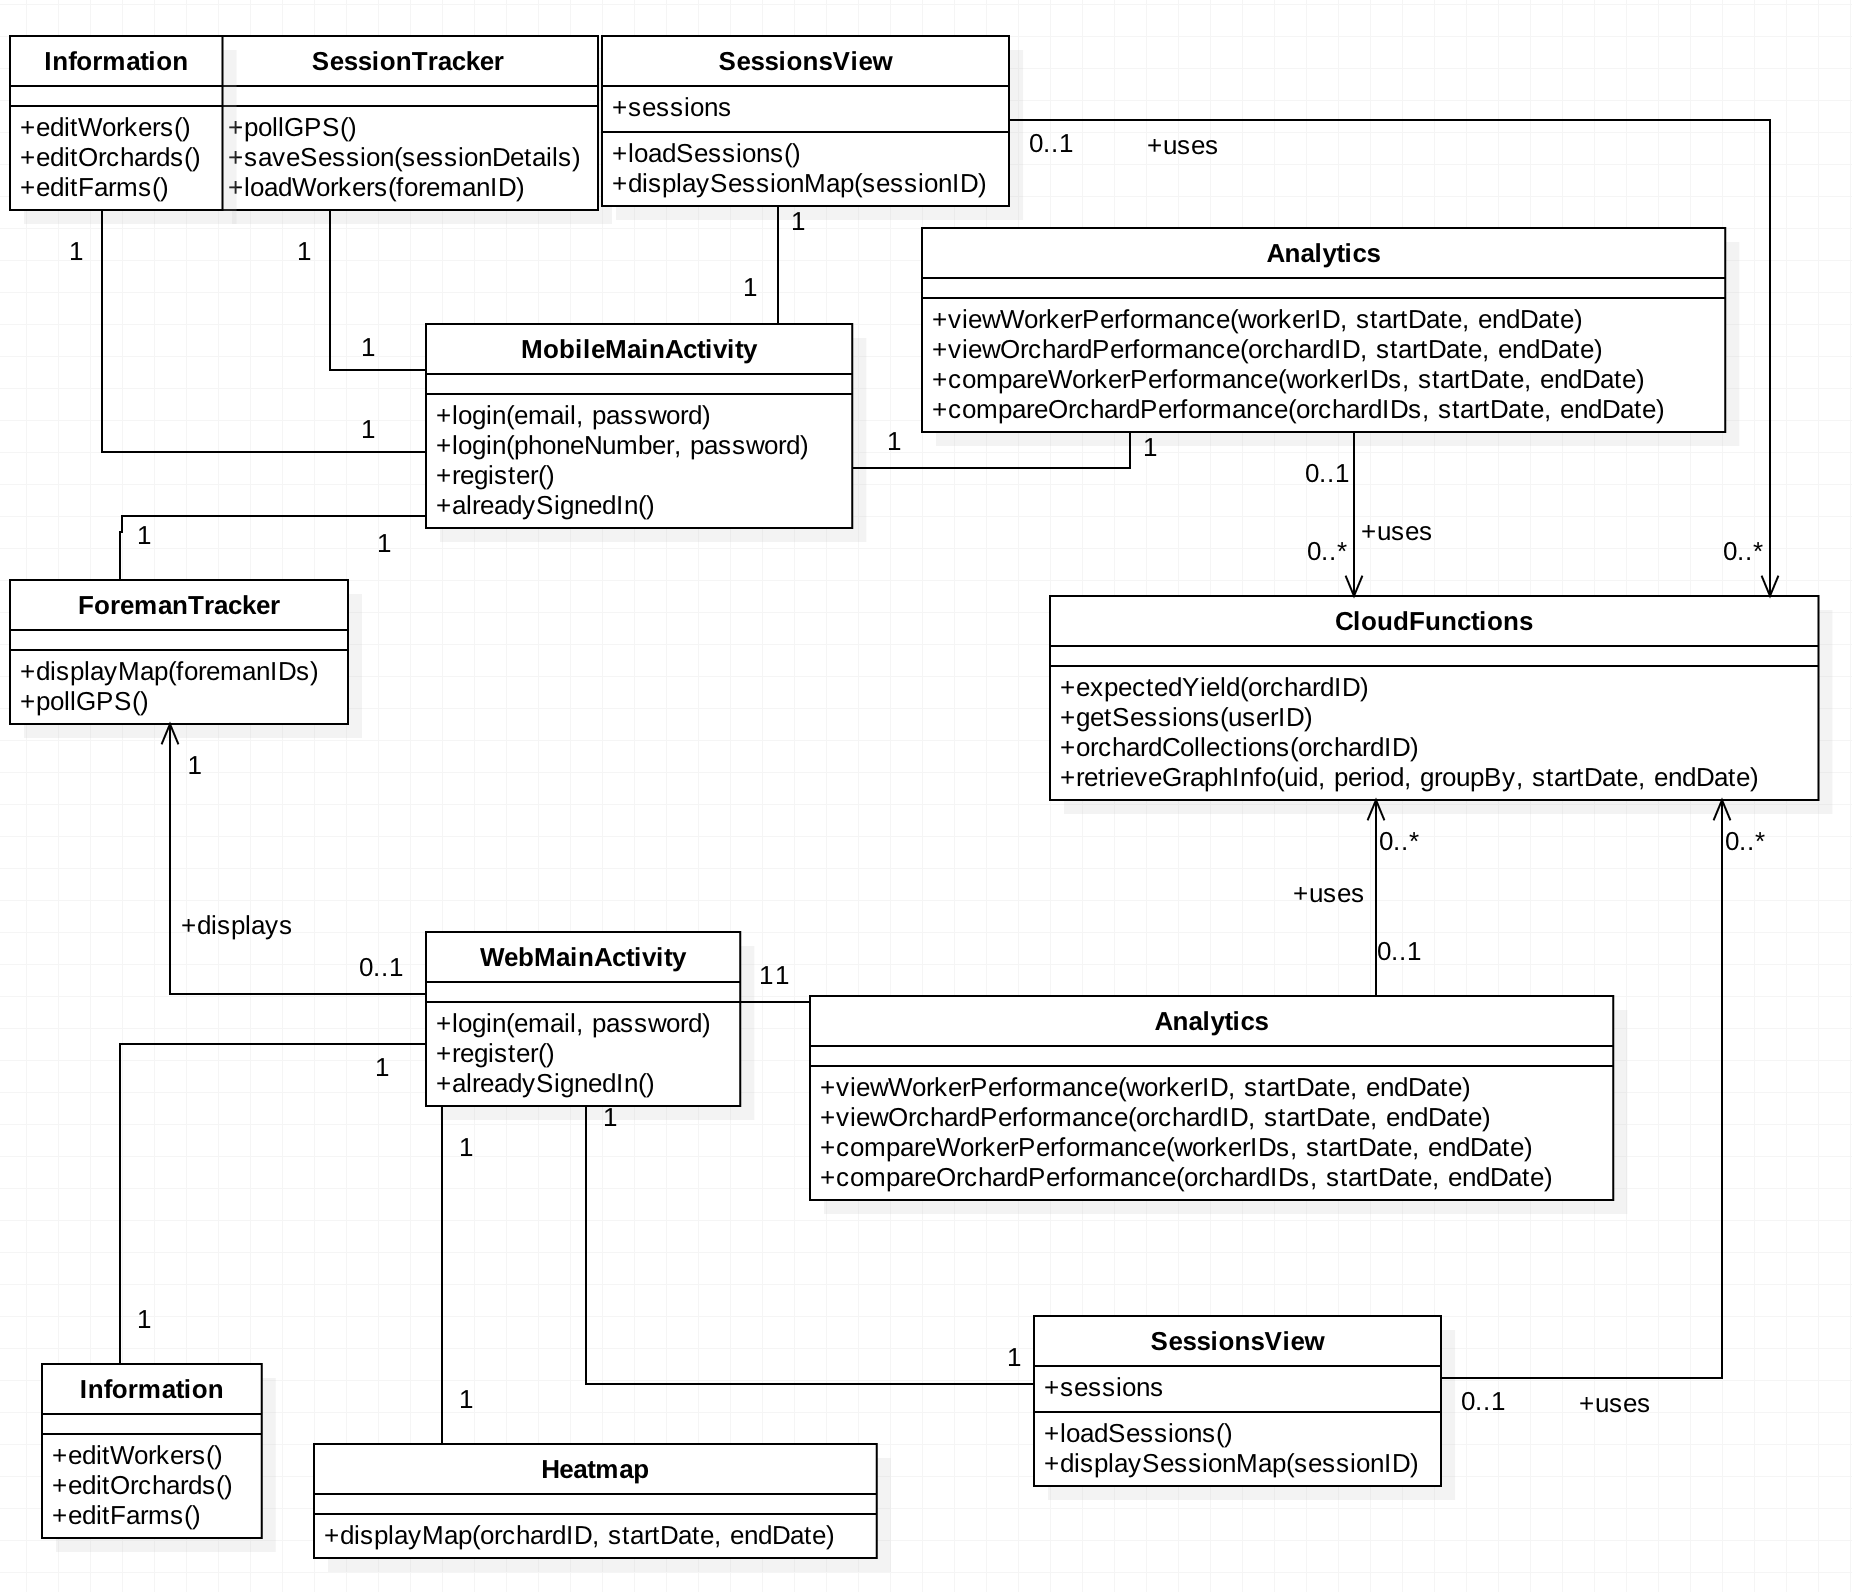
\includegraphics[width=1.2\linewidth]{UMLClassDiag.png}

\center{\section{Functional Requirements:}}
\flushleft{\subsection{Users}
Need information here.
}
\flushleft{\subsection{Subsystems}
Need information here.
}
\subsection{Specific Requirements}
  \flushleft{\item[$\bullet$]On sign in Harvest shall verify credentials against the database before signing them in. 
  \item[$\bullet$]Harvest shall create a profile on the database for the user through a registration form.
  \item[$\bullet$]Harvest shall measure yield through the input view of the mobile interface.
  \item[$\bullet$]The Harvest mobile interface shall make use of GPS data and based on weight and location assumptions, it must give approximate yield estimates not only for each orchard, but for each approximate location where the data was entered.
  \item[$\bullet$]The Harvest system shall make use of analytics to measure worker performance.
  \item[$\bullet$]The Harvest website shall display heat map data, showing the locations in which the most yield has been collected.
  \item[$\bullet$]The Web interface shall show detailed information about produce. (e.g. cultivar, year planted).
  \item[$\bullet$]The Harvest system shall do administrative tasks through the web interface.
  \item[$\bullet$]The Harvest website shall give the farmer/administrator a real time map view of the foreman's location.
  \item[$\bullet$] Both foremen and farmers shall have access to the mobile interface, with foremen unable to carry out any administrative changes or view analytical data on it.
  \item[$\bullet$] Only farmers shall make use of the website, as it is designed to track their workers, foremen and measure performance in and around their farms.
}

\center{\section{Non-functional Requirements}}
\flushleft{Need information here} \newline

\center{\section{System Architecture}}
\flushleft{\subsection{Determining Design Objectives}}
\flushleft{\item[$\bullet$] The design is aimed to provide accessibility, data integrity and optimize performance.
\item[$\bullet$] The design is also aimed at producing a user friendly easy to use system.
\item[$\bullet$] The design is aimed at easing facilitation and automation of work. 
\newline
}


\flushleft{\subsection{Interfaces}}

\flushleft{\subsubsection{User Interfaces:}
\textbf{The Application Interface: }This interface will have the functionality for login in and signing up of foremen. It will have yield data recording functionality and worker performance capturing functionality. \newline
\textbf{The Web Application Interface: }The administrative tasks will be carried out on the Interface (Like adding worker and Orchard Details per farm), as well as tracking of workers and performance. \newline
}
\textbf{The Database Interface: }This interface will maintain strict access, it will only be accessed through an abstract interface (Backend) only to store and retrieve data. \newline
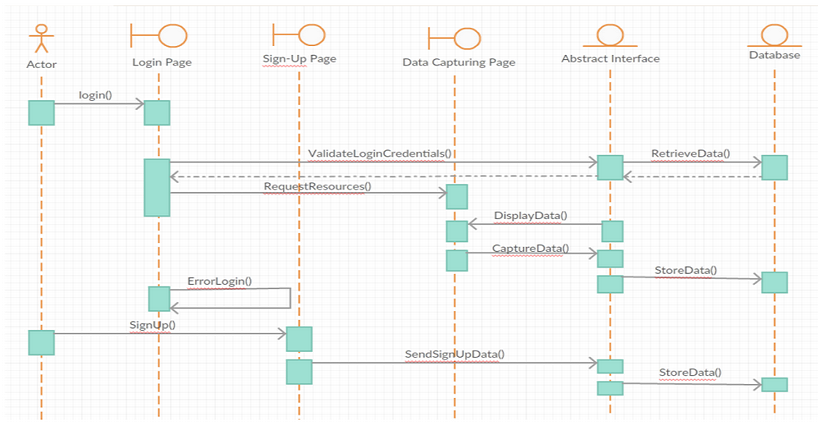
\includegraphics[width=1.2\linewidth]{sequenceDiag.PNG}

\flushleft{\subsubsection{Hardware Interfaces:}
Need information here. \newline
}
\flushleft{\subsubsection{Software Interfaces:}
Need information here. \newline
}

\subsection{Architectural Styles}
\flushleft{
The architectural structural design of our the Harvest system is a Persistence Framework. The system has 3 main subsystems (Android Application, IOS Application and the website) all heavily reliant on the database system providing them with efficient object storage and retrieval without the need for implementation detail. It also hides the database details such as implementation from the subsystems, and  therefore uses an abstract interface to manipulate data. 
}

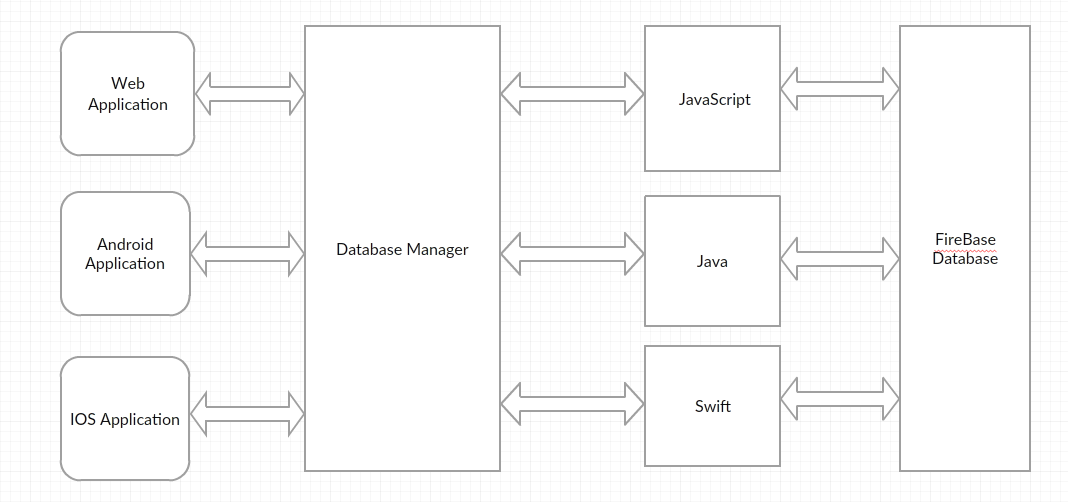
\includegraphics[width=1.0\linewidth]{persistenceFrameWork.PNG}

\flushleft{\subsubsection{Reviewing the Architectural Design}
\item[$\bullet$]The Harvest application is accessible from a smartphone/tablet/desktop computer.
\item[$\bullet$]The Harvest system checks whether the user is registered before signing them in. 
\item[$\bullet$]Harvest creates a new profile of the user when registering them.
\item[$\bullet$]Harvest measures yield through the input view of the mobile interface.
\item[$\bullet$]Harvest does facilitate GPS data filtering and Web Functionality.
\item[$\bullet$]The software application does facilitate the idea of tracking.
}

\flushleft{\subsection{System Configuration}
\subsubsection{Technology Used}
\item[$\bullet$]Database System : Firebase
\item[$\bullet$]IDE's: Xcode, Android studio
\item[$\bullet$]Programming languages: XML (Android UI); Java (Android Backend); Swift (IOS); HTML, CSS, JavaScript (Website)
}
\flushleft{\subsubsection{Deployment Diagram}
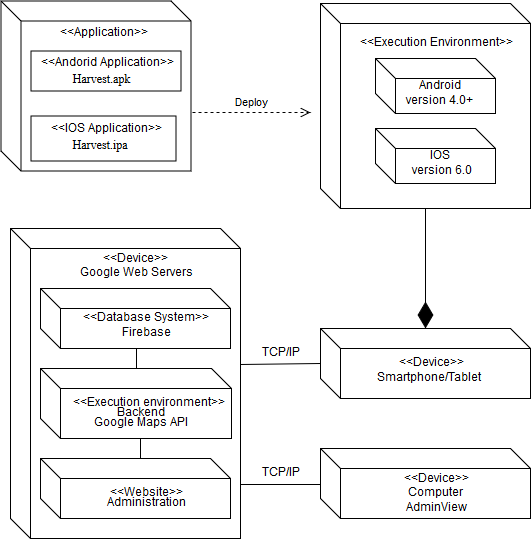
\includegraphics[width=.85\linewidth]{deployment.png}
}

\end{document} 